\documentclass[acmsmall, nonacm]{acmart}

\usepackage[utf8]{inputenc} % allow utf-8 input
\usepackage[T1]{fontenc}    % use 8-bit T1 fonts
\usepackage{hyperref}       % hyperlinks
\usepackage{url}            % simple URL typesetting
\usepackage{booktabs}       % professional-quality tables
\usepackage{amsfonts}       % blackboard math symbols
\usepackage{nicefrac}       % compact symbols for 1/2, etc.
\usepackage{microtype}      % microtypography

\usepackage{amsmath,amssymb}
\usepackage{graphicx,grffile}

\usepackage{longtable}
\usepackage{subcaption}
\usepackage{xcolor}


\title{State description language and PathRL notes}

% XXX contributors' macros
% gleb
\newcommand{\GG}[1]{\textcolor{red}{[GG: #1]}}
% daniil
\newcommand{\danil}[1]{{\color{red} [#1]}}
% ivan
\newcommand{\attn}[1]{{\color{magenta}{\textbf{#1}}}}


\begin{document}

\maketitle

\section{Scattered thoughts} % (fold)
\label{sec:scattered_thoughts}

In this section we collect ideas and though that might be interesting to discuss or
experiment with.
% 
\attn{
I think the ideal situation would be to have to versions of the codebase:
``educational'' and ``massive''.
%
The first illustrates the idea and the logic of the method on a toy environment,
follows the notation of the paper, runs serially and requires but a single GPU
(not a compute cluster and without multiprocessing, MPI or Horovod nightmarish
clutter).
% 
The second is used to make massive experiments to achieve SOTA or test complex
environments and thus allowed to conceal the method's logic behind the spaghetti
of parallelization.
}

% attention, motivation (self-awareness + focus + goal) -- self-motivation
%  rational sub-goals -- inferred from the current state given the overall motivation

\section{World models with inverse dynamics and autoencoders} % (fold)
\label{sec:wm_idm_ae}

We could try to fuse a world model with the inverse dynamics model. Let $W$ be a
world model that maps the current state and action to a potential next state: $
    \hat{s}_{t+1} = W(s_t, a_t)
$. However, since we \emph{know} that the environment is stochastic and its state
$s_t$ contains either irrelevant or uncontrollable information, it seems crucial to
pull the world model back to the latent variable level: $
    \hat{z}_{t+1} = W(z_t, a_t)
$, where $z_t$ are devoid of \emph{irrelevant} information. To this end consider
the following structure, which is borrowed from the work by \citet{watter_embed_2015}:
\begin{align*}
    a_t &\sim c(\phi(s_t), \phi(s_{t+1}))
        &\text{ Siamese IDM and attention-based vAE train } \phi
    \,, \\
    s_t &\sim \psi(\phi(s_t))
        &\text{ learnt using attention-based vAE}
    \,, \\
    \hat{z}_{t+1}
        &= W(z_t, a_t) \big\vert_{z_t = \phi(s_t)}
        &\text{ WM dynamics (embed to control)}
    \,, \\
    \hat{z}_{t+1}
        &\sim \phi(s_{t+1})
        &\text{ predicted embeddings should be relevant}
    \,, \\
    s_{t+1}
        &\sim \psi(\hat{z}_{t+1})
        &\text{ reconstruction with attention}
    \,.
\end{align*}
We might want to infer an attention mask $\alpha_t = \alpha(\phi(s_t), \phi(s_{t-1}))$
when reconstructing the state with $\psi$, trained with attention-based vAE using
MAX-ENT regularizer on the attention, like in \citep{choi_contingency-aware_2019},
or other denoising cycle-consistency imposing method on $\phi-\psi$ pair, akin to
CycleGAN.

% \href{https://arxiv.org/abs/2102.11329.pdf}{2102.1132}

% subsection scattered_thoughts (end)

\section{Go-Explore extended review}

We begin with a long winded extended review of the Go-Explore framework proposed by
\citet{ecoffet_go-explore_2021} and \citet{ecoffet_first_2021}.
% 
\attn{This will be definitely rewritten, because the reviewed papers could have been
written more concisely and overall better organized by their authors.
%
I just wanna read something else atm, to clear the mind. Their code is as all over
the place as their paper.
}

\medskip
% motivation and how it works
Intrinsic motivation via augmented rewards has drawbacks, that limit its ability to
explore promising states. Namely, \emph{detachment} and \emph{derailment}.
%
Roughly, a state's curiosity potential measures how often it has been frequented. Hence
an intrinsically motivated agent can, in principle, pathologically deplete curiosity
around itself or along a ``narrow passage'' through an \emph{eye-of-a-needle} state,
thereby prohibiting itself from revisitng prior underexplored states. The agent thus
becomes disconnected, or \emph{detached}, from the frontiers of high intrinsic reward,
especially when the exploration is restarted from a small set of initial states.
% XXX intrinsic reward regeneration? curiosity is a consumable resource.
%
\emph{Derailment} takes place when the policy that tries to return to a promising state
and explore it further gets distracted or stochastically perturbed along the way, thereby
not arriving at the desired goal.
%
For example, intrinsic motivation make the agent return to exploration-worthy states,
however the epsilon-greediness, action noise or network stochasticity force them to
explore while doing so. If we could turn exploration off for the duration of ``returning'',
then there would be no derailment. In other words, having high propensity to explore
in unknown areas, and low -- in well-known areas, would eliminate derailment.
%
% XXX bayesian networks and deep uncertainty estimation?
It is worth noting, that a deep networks are usually overconfident on out-out-distribution
inputs, and thus are unlikely to have the expected levels of uncertainty in poorly explored
states, \citep[p.~34]{ecoffet_first_2021}.  % hence they make sure to use maxent regularizer.

\citet{ecoffet_go-explore_2021} propose the Go-Explore framework for hard-exploration
problems that produces high-return trajectories useful for training better RL agents
via imitation learning.
% >>>  appears to be especially powerful, suggesting
%     it may be fundamental feature of learning in general, \citep[p.~12]{ecoffet_first_2021}.
%
Go-Explore framework claims to solve derailment and detachment by decomposing exploration
into three components: remembering previously found states with high exploration potential,
returning to them and then exploring from them. When returning to a state it is possible
to leverage domain knowledge, technical capabilities of the environment, or auxiliary agents,
e.g. level coordinates, simulator save sates, or special return policies.

Specifically, \citet{ecoffet_go-explore_2021} propose two phases.
% 
During the \emph{GO-EXPLORE} phase we find a solution that works barely, kind-of, or
very suboptimally, but nevertheless works and achieves high cumulative reward albeit
under restrictive assumptions.
% XXX Do we learn in gex phase or just explore? (just explore, unless we are training
%     a return policy).
% >>> If we can handle stochasticity and learn goal-conditioned policies, then the robustify
%     phase might not be necessary.
% XXX Isn't the goal privileged info?
% 
At the \emph{robustify} phase this \emph{brittle} solution is improved by making it
resilient against environmental adversity and chance, to ensure that it is capable of
consistently achieving similar performance.
% >>> robustification phase is good at fine-gradined optimisation, while the exploration
%     phase biases the collection of trajectoreies towrads higher scoring ones

At the \emph{GO} step we return the agent to a promising state, a ``stepping-stone'',
without any exploration.
%
The state-to-return is randomly picked from the state-archive, with chances determined
by ``promise'' scores. To achieve this it \citep[app.~A.5]{ecoffet_go-explore_2021} uses
general heuristics, e.g. the state visitation metric, or more domain specific, like the
number of seen neighbours and distance from the initial state.

The cells, i.e. low-dimensional hashes of the observations, clusters, are used as keys
in the archive. However, their hyperparameters are not fixed and instead are adjusted
during the go-explore phase at regular intervals to minimize some metric
\citep{ecoffet_first_2021}. The adjustment is sampled from geometric distributions
around the best current parameters and aims at improving the cell distribution in
the archive based on the normalized entropy $
    H(p; \theta)
        := \frac{\mathbb{H}(p)}{\log n}  % {- n \frac1n \log \frac1n}
$ and the discrepancy of the number of cells \citep[p.~15-16]{ecoffet_first_2021}. All
of this is run on a set of the most recently seen unhashed observations with capacity
of $10$k samples.
% 
They also use a special virtual cell tracking the episode termination,
\citep{ecoffet_first_2021}.

Returning to a good state itself hinges on the ability to replay a sequence of actions in
the environment and end up exactly is the final state of the recorded trajectory. This
requires that during the \emph{GO}-step the environment be deterministic, which although
unrealistic, can still be used, since it does not really matter in the end what divination
was employed during training of a well performing agent or what privileged information or
setup used to steer it to a better local minimum, obviously if the environment or simulation
readily permits that. However in their subsequent work \citep{ecoffet_first_2021} address
this ``trick'' by using \emph{goal-conditioned} policies to make the go-explore phase able
to handle training in stochastic environments.

Having returned to a ``good'' state we proceed with the \emph{EXPLORE}-step.
%
Exploration in their paper is completely stochastic, e.g. random actions are sampled
for a set duration or until termination. Every state in the archive has the action-state
trajectory, the environment save state, the cumulative reward and length. New states
are added straightforwardly, whereas existing states are updated only if the old one
is lexicographically worse than the new one w.r.t. pairs ``(cumulative score, negative
length)''. Visitation counters are \emph{not} reset, and the random exploration is run in parallel.

The \emph{robustification} phase learns from explored demonstrations to imitate the best
performing trajectories from the archive (preferably from non-overlapping explore phases)
so far in when the stochasticity is injected back into training. They assume that it would
be easier to improve a good demonstration policy, rather than learn a new one in sparse
or deceptive reward setting.
% 
% datasets contain the demonstration trajectories.
%
This phase uses a batched modification of the Backward algorithm of \citet{salimans_learning_2018},
\citep[app.~A.7]{ecoffet_go-explore_2021}.
%
Starting from $s_t$ in a trajectory $\tau = (s_t, a_t)_{t=0}^T$ it trains the agent until
its cumulative reward in the environment exceeds that of the demonstration, then moves back
the initial state to $s_{t-1}$ and repeats the cycle (work back from $s_{T-1}$ until $s_0$
is reached). The modification backtracks to a state from a demonstration chosen at random
from the given pool.
% XXX how is this cumulative reward measured? the env is assumed to be stochasitic at
%  this phase.
Placing the agent at an initial state $s_t$ requires resetting the environment to that state
\citep[L.~28 of alg.~1]{salimans_learning_2018}. Presumably, \citep{ecoffet_first_2021} use
either the return policy in stochastic environments or save-states in deterministic ones.

This phase makes the agent learn to imitate and improve the given demonstrations by running
a blend of PPO \citep{schulman_proximal_2017} and SIL \citep{oh_self-imitation_2018}: some
agent instances act in the environment and are optimized via PPO, while others designated
as SIL agents replay the actions from a given trajectory pool. Robustification phase
hyperparameters are given at \citep[p.~30]{ecoffet_first_2021}.
%
% XXX it seems that the BA does not handle rnn hidden states well.
% XXX rnn hidden states can be reshaped into 2d memory-like with random access
%
The robustification phase makes a checkpoint every $100$ iterations and afterwards selects
the best-performing policy among those with the highest rolling average training score
by evaluating them for $100$ episodes in a test environment, \citep{ecoffet_first_2021}.
This best policy is re-tested for $1000$ episodes to eliminate selection bias in reporting.

The go-explore archive was pre-filled from up to 15 billion steps prior to the first
robustification phase \citep[p.~19]{ecoffet_first_2021}.

Training stochasticity in Atari games can be brought back either by performing a random
number of \emph{NOP}-s after each restart, or by introducing ``sticky actions'', which
inject extra stochasticity into the environment dynamics through imprefect action control
(``shaky hand''), which mimics a non-frame perfect player by randomly ignoring the newly
issued command and repeating the previous input instead.
% >>> Community guidelines advocate sticky actions as a way to evaluate agents on Atari3,
%     and there is substantial evidence to show that sticky actions can decrease performance
%     substantially compared to the now deprecated no-ops evaluation strat- egy3,45,46.

% XXX Their truly remarkable achievement is Pitfall. Is it though? What about
%  other simpler games?
% XXX how well does GO-EXPLORE fare in partially observed MDP?
Exploitation of determinism coupled with ``deceptive'' rewards in the Go-Explore phase
may lead to what they call ``busy highway problem'', in which the solely due to determinism
the non-viable trajectories, like crossing the highway directy, not detouring via a bridge,
become the only ones that make it to the robustification phase
\citep[p.~17]{ecoffet_go-explore_2021}.
% 
The examples of deceptive rewards include: euclidean distance to the coffee machine during
training of a household service robot does not reflect the topography and completely
neglects obstacles, or high penalty for self-damage that prevent a rescue robot from
exploring the area for survivors.

% XXX do they use allow feedback from the robustification phase? Is the learnt network
%  ever used anywhere besides phase 2?

Goal-conditioned return policy of \citet{ecoffet_first_2021} (policy-based go-explore)
enables returning to the specified state in environments, which are inherently stochastic
instead of using save-states. Although this makes the method less efficient, still
the return policy can be used to sample new actions and goals during exploration, by
leveraging its generalization ability \citep[p.~38]{ecoffet_first_2021}.
% 
Conditioning is done directy by concatenating the cell-representation of the goal, i.e.
the cell of the state to return to.
% >>> Instead, the actor is iteratively conditioned on the successive cells traversed
%     by the archived trajectory that leads to the goal cell.
% \citep{guo_self-imitation_2019} soft-order trajectory, i.e. when training in each
%     batch it uses $s_t$ and $cell(s_{t+1})$ as inputs to the policy
%     (baby-steps, forward HER). The successive cells are deduplicated, and the number
%     of real steps (intermittent states) is counted.
% XXX we can use Hindsight Experience Replay here.
% 
% XXX \citep{schulman_proximal_2017}
%   reinforce-pg (ppg-clip with GAE) + ell_2-vf + negent + ell-2-param + SIL
The policy is trained with actor-critic-style PPO \citep{schulman_proximal_2017} during
the \emph{exploration} phase (after the ``go'' step), and its policy temperature, i.e.
the pre-softmax logit divisor, is increased if the agent takes too long to reach the next cell,
\citep[p.~19]{ecoffet_first_2021}.
% 
The goal-conditioned policy is trained to follow the best trajectory of states that
previously led to the selected state from the archive and also undergoes self-imitation
learning \citep{oh_self-imitation_2018} (also used in \textbf{robustification} phase).
The SIL loss is computed over the $(s, a, G)$ sequences from past trajectories ($G$ is
the present value of rewards following the state $s$).
% XXX actions are replayed in the environment?

With SIL the batch is spliced
from two sources: the current policy and the pre-recorded trajectory:
$$
    \beta \underbrace{\mathbb{E}_{s, a\sim p_{\pi_{\theta_-}}(s, a)}
            \biggl\{
                \frac{\pi_\theta(a\mid s)}{\pi_{\theta_-}(s, a)} \cdots
            \biggr\}
    }_{\text{PPG}}
    + (1 - \beta) \underbrace{
        \mathbb{E}_{s, a\sim \hat{D}}
        \Bigl\{
            \log \pi_\theta(a \mid s) \cdots
        \Bigr\}
    }_{\text{SIL --- PG}}
    \,. $$

As soon as the training reached the last cell of the trajectory, the agent switches to
the \emph{explore} step, which is either policy- or random- exploration. For policy
exploration it picks either a synthetic goal-cell, or a neighbouring cell or an arbitrary
cell from the archive. Whenever the set goal is reached or the steps runs out, then a
new goal is picked, \citep[p.~21]{ecoffet_first_2021}.

\medskip
% \citep{salimans_learning_2018} is like HER but without goals:
%  it gradually backtracks the initial state from the end of the trajectory to its beginning.
%  The agent learns to improve the reward (as measued in where?) and then the initial state
%  is moved one step earlier.
% See also \citep{resnick_backplay_2018}.
% 
% XXX Although exploration is random, the overall population of trajectories in
% the archive is guided by the ``promise'' score.
%
% XXX isn't this sort of like a genetic algorithm? without corssing-over or mutation,
%  just splicng new action sequences to the existing promising ``strand''? But its
%  cheap, since it does not require computed interactions, just sampling. It works
%  better than random search precisely because we can ``return'', i.e. build upon
%  the existing strand well perfroming trajectory.
% XXX modified perferential evolutionary search. Apparently it is called quality diversity
%  algorithms (MAP-elite) \citep{mouret_illuminating_2015}

% XXX Who cares how the agent was trained, with or without smilation resets, save
%  states or whatever, as long as it performs well in evaluation environments.
% If we can leverage determinism, when training why not? We just need to make sure
%  that we account and make the learnt model robust against noise.

%  to provide a method for more effective exploration
% what are their contribs
% how are relevant to us
% * two phases: go-explore and robustify
%   1. remember previously visited states
%   2. return to a promising state w/o exploration and explore from it
%   3. solve through exploiting, then robustofy through imitation
% * go-explore produces many high-perfoming demonstrations automatically and cheaply

% XXX isn't their ``archive of states'' essentially another name for a value function?
%  stemming not form bellman operator, but something else? yes but it must be easily
%  ``searcahble'', or at least handle the ``max-query'', and ``resettable''.
% XXX archive (with cells) is a keyed-storage -> looks like a tabular method. Why not
% a functional approximation (like soft hashing of the states, or soft-ranking)? $
%   f\colon \mathcal{S} \to \mathbb{R}
% $. With updates
%  and resets? But we will need to search through it. Searchable deep funciton
%  with crisp enough states that it can be reliably ``returned to''.
% XXX sponge, squeeze it to get gunk.

% contrast with intrinsic motivation
In light of \citep{silver_reward_2021} it is the reward signal (extrinsic or emergent)
that actually causes targeted and well-explored behaviour, rather than an algorithm.


\begin{figure}
% XXX All artwork must be neat, clean, and legible. Lines should be dark
%  enough for purposes of reproduction. The figure caption should be lower
%  case (except for first word and proper nouns)
% You may use color figures.  However, it is best for the figure captions and the
% paper body to be legible if the paper is printed in either black/white or in
% color.
  \centering
  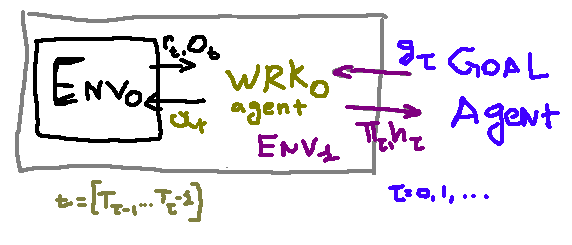
\includegraphics[width=0.9\linewidth]{./assets/ga_wrk_hierarchy.png}
  \caption{
  \emph{Layers of abstraction (encapsulation)}:
  the goalsetter treats the worker in its environment jointly as a single
  black-box (non-diff'able with internal time-scale $t$) environment with
  states $h_\tau$, rewards $pi_\tau$ and goals $g_\tau$ as control.
  % 
  \attn{crude sketch. MAYBE an ``onion'' with the goalsetter at the core?}
  }
  \label{fig:environment_hierarchy}
\end{figure}

\section{Additional reviews}

\medskip

% this should be rewrtitten, as it does not answer any review question:
%  contributions, relevance, criticism
A triplet of papers \citep{hafner_learning_2019,hafner_dream_2020,hafner_mastering_2020} propose
to learn the optimal control policy via dynamics in the latent space, wherein a stochastic
model of the world is identified and the agent learns its policy using the analytical
gradients through the learnt dynamics and reward function.
%
In \citep[alg.~1]{hafner_dream_2020} the training alternates between learning latent dynamics
and observation-to-latent representations, and optimizing the policy in the latent space of
the \emph{virtual} environment determined by the identified ``world model''.
% iterative learning control
The world model is trained from experience and the policy is trained with a frozen world model.

During the second phase experience is collected in the real environment (how?)
% act out the learnt policy in the real env through the representation model.

The model of the ground-truth environment is that of the partially observed MDP (incomplete
information) with the following
\begin{align*}
  a_t & \sim p(a \mid o_{\leq t}, a_{< t})
    \,, \\
  o_{t+1}, r_{t+1}
    & \sim p_t(o, r \mid o_{\leq t}, a_{< t}, a_t)
    \,,
\end{align*}
where non-stationarity of $p_t$ is due to the unobserved true full state of the environment.
% 
The proposed world model is
\begin{equation*}
  \begin{aligned}
    & \text{representation model}
      & & h_{t+1} \sim p(h \mid h_t, a_{\leq t}, o_{\leq t})
          \,, \\
    & \text{transition dynamics}
      & & h_{t+1} \sim q(h \mid h_t, a_t)
          \,, \\
    & \text{rewards}
      & & r_{t+1} \sim q(r \mid h_{t+1})
          \,, \\
  \end{aligned}
\end{equation*}
and the agent's policy (and value for actor-critic) depends on the inferred latent state $
  a_t \sim \pi(a\mid h_t)
$. The model is designed in such way that it is possible to differentiably sample from it.

The policy is learnt using the imagined trajectories cast from the current state of the 
ground-truth environment: infer the recent latent state $h_t$ from the history $
  (o_s, a_s, r_s)_{s \leq t}
$ and ``dream'' latent differentiable trajectories from it $
  (h_\tau, a_\tau, r_\tau)_{\tau \geq t}
$ with $a_\tau \sim \pi(a\mid h_\tau)$ and the transition and reward dynamics. The agent
maximizes $
  \mathbb{E}_{\pi}^{\geq t} \bigl\{
      \sum_{s \geq \tau} \gamma^{s - \tau} r_s
    \bigr\}
$ using path derivatives rather than score-function approach.
% 
Since we backprop through a recurrent system, the we face the issue of exploding, of
vanishing gradients, if the largest-magnitude of eigenvalue of the latent-to-latent
Jacobian is not away from the the unit circle.

It might be useful to treat this as sort of ``seq-to-seq'' training where we learn
a policy $\pi$ on the latent state to maximize the sequence of returns or Generalized
Advantage Estimates, \citep{schulman_high-dimensional_2016}. Since reducing the while
future trajectory since $\tau$ just to as single return $G_\tau$ might result in poor
credit assignment.

The imaginary world model is trained using the ELBO \attn{what variational approximations?}.
\footnote{
  The inference engines $q$ as opposed to models $p(O, A)$, with the former approximating
  the model-based posterior.
}
%
The policy is parameterized by
$$
a = \tanh\Bigl(\mathcal{N}\bigl(
    \mu(h), \operatorname{diag}{\sigma^2(h)}
  \bigr)\Bigr)
  \,. $$


\citet{chen_decision_2021} appeal to the upside-down RL paradigm and treat the task as
a large seq-to-seq learning task. The most interesting piece is conditioning the action
taken on the desired return from taking the action and following some generalized policy
later on.

% XXX what is a plan? can we create ``options'' on-the-fly and enrich the action space
%  with them? DO we need specia lagos for this, or the PPO, A2C of the good'ol DQN could
%  do the trick? ?

\section{What is this?}

\paragraph{What is this?} % (fold)
\label{par:what_is_this}

This has been copied from some old notebook of mine that had no context. It appears to be
related to PPO, \citep{schulman_proximal_2017}, and ENAS.
%
Policy-gradient (non-rigorous):
$$
L^\text{PG}(\theta)
    := \hat{\mathbb{E}}_t
        \log \pi(a_t\mid s_t; \theta) \widehat{A}_t
    \,. $$
Importance weight for old-vs-current policy
$$
w_t(\theta)
    := \frac{\pi(a_t \mid s_t; \theta)}{\pi(a_t \mid s_t; \theta_-)}
\,. $$
TRPO (non-rigorous):
$$
\begin{aligned}
    &\underset{\theta}{\text{maximum}}
      & &
        \hat{\mathbb{E}}_t w_t(\theta) \widehat{A}_t
        \,, \\
    & \text{subject to}
      & & \hat{\mathbb{E}}_t
        \operatorname{KL}\bigl(
            \pi(\cdot \mid s_t; \theta)
            \| \pi(\cdot \mid s_t; \theta_-)
        \bigr) \leq \delta
    \,.
\end{aligned}
    $$
But constrained optimization is ``hard'' in TRPO, so PPO uses the regularized objective.
% 
The current policy loss
$$
L(\theta)
    := \hat{\mathbb{E}}_t w_t(\theta) \widehat{A}_t
    \,. $$
The clipped-ratio policy loss
$$
L^\text{CLIP}(\theta)
    := \hat{\mathbb{E}}_t \min\bigl\{
        w_t(\theta) \widehat{A}_t,
        \operatorname{clip}(w_t(\theta), 1 - \varepsilon, 1 + \varepsilon) \widehat{A}_t
    \bigr\}
    \,, $$
where $\operatorname{clip}$ removes the incentive for moving $w_t(\theta)$ away from one,
and $\min$ makes the objective into a lower bound on $L(\theta)$.

Policy loss with KL-penalty
$$
L^\text{KLPEN}(\theta)
    := L^\text{CLIP}(\theta)
    - \beta \, \hat{\mathbb{E}}_t
        \operatorname{KL}\bigl(
            \pi(a \mid s_t, \theta_-)
            \| \pi(a \mid s_t, \theta)
        \bigr)
    \,, $$
uses adaptive regulator for $\beta$ when the Kullback-Leibler divergence ``exceeds''
($\times 2$ if $> d_\text{trg} \frac32$) or ``undershoots'' the target ($\div 2$
if $< d_\text{trg} \frac23$).

Negative to what is computed in \texttt{PPO.policy\_loss}
\begin{align}
\max_\theta L^\text{enas}(\theta)
    &= L^\text{CLIP}(\theta)
        + (\mathrm{entropy\_coef})\, \hat{\mathbb{E}}_t \mathbb{H}(\pi(a_t\mid s_t, \theta))
    \\
        &+ \beta \underbrace{
            \mathbb{E}_{a\sim \pi(a \mid s_t, \theta_-)} \log \pi(a \mid s_t, \theta)
        }_{\text{what is left of KL}}
    \,.
\end{align}
Everywhere $\hat{\mathbb{E}}_t$ is average over the sample $
    S_t = (a_{ti}, s_{ti}, \widehat{A}_{ti})_{i=1}^m
$.

% paragraph what_is_this (end)

\bibliographystyle{abbrvnat}
\bibliography{references}

\end{document}